\documentclass[twoside]{book}

% Packages required by doxygen
\usepackage{fixltx2e}
\usepackage{calc}
\usepackage{doxygen}
\usepackage[export]{adjustbox} % also loads graphicx
\usepackage{graphicx}
\usepackage[utf8]{inputenc}
\usepackage{makeidx}
\usepackage{multicol}
\usepackage{multirow}
\PassOptionsToPackage{warn}{textcomp}
\usepackage{textcomp}
\usepackage[nointegrals]{wasysym}
\usepackage[table]{xcolor}

% Font selection
\usepackage[T1]{fontenc}
\usepackage[scaled=.90]{helvet}
\usepackage{courier}
\usepackage{amssymb}
\usepackage{sectsty}
\renewcommand{\familydefault}{\sfdefault}
\allsectionsfont{%
  \fontseries{bc}\selectfont%
  \color{darkgray}%
}
\renewcommand{\DoxyLabelFont}{%
  \fontseries{bc}\selectfont%
  \color{darkgray}%
}
\newcommand{\+}{\discretionary{\mbox{\scriptsize$\hookleftarrow$}}{}{}}

% Page & text layout
\usepackage{geometry}
\geometry{%
  a4paper,%
  top=2.5cm,%
  bottom=2.5cm,%
  left=2.5cm,%
  right=2.5cm%
}
\tolerance=750
\hfuzz=15pt
\hbadness=750
\setlength{\emergencystretch}{15pt}
\setlength{\parindent}{0cm}
\setlength{\parskip}{0.2cm}
\makeatletter
\renewcommand{\paragraph}{%
  \@startsection{paragraph}{4}{0ex}{-1.0ex}{1.0ex}{%
    \normalfont\normalsize\bfseries\SS@parafont%
  }%
}
\renewcommand{\subparagraph}{%
  \@startsection{subparagraph}{5}{0ex}{-1.0ex}{1.0ex}{%
    \normalfont\normalsize\bfseries\SS@subparafont%
  }%
}
\makeatother

% Headers & footers
\usepackage{fancyhdr}
\pagestyle{fancyplain}
\fancyhead[LE]{\fancyplain{}{\bfseries\thepage}}
\fancyhead[CE]{\fancyplain{}{}}
\fancyhead[RE]{\fancyplain{}{\bfseries\leftmark}}
\fancyhead[LO]{\fancyplain{}{\bfseries\rightmark}}
\fancyhead[CO]{\fancyplain{}{}}
\fancyhead[RO]{\fancyplain{}{\bfseries\thepage}}
\fancyfoot[LE]{\fancyplain{}{}}
\fancyfoot[CE]{\fancyplain{}{}}
\fancyfoot[RE]{\fancyplain{}{\bfseries\scriptsize Generated on Sat Dec 12 2015 01\+:21\+:31 for C\+I\+S\+C475-\/\+P5 by Doxygen }}
\fancyfoot[LO]{\fancyplain{}{\bfseries\scriptsize Generated on Sat Dec 12 2015 01\+:21\+:31 for C\+I\+S\+C475-\/\+P5 by Doxygen }}
\fancyfoot[CO]{\fancyplain{}{}}
\fancyfoot[RO]{\fancyplain{}{}}
\renewcommand{\footrulewidth}{0.4pt}
\renewcommand{\chaptermark}[1]{%
  \markboth{#1}{}%
}
\renewcommand{\sectionmark}[1]{%
  \markright{\thesection\ #1}%
}

% Indices & bibliography
\usepackage{natbib}
\usepackage[titles]{tocloft}
\setcounter{tocdepth}{3}
\setcounter{secnumdepth}{5}
\makeindex

% Hyperlinks (required, but should be loaded last)
\usepackage{ifpdf}
\ifpdf
  \usepackage[pdftex,pagebackref=true]{hyperref}
\else
  \usepackage[ps2pdf,pagebackref=true]{hyperref}
\fi
\hypersetup{%
  colorlinks=true,%
  linkcolor=blue,%
  citecolor=blue,%
  unicode%
}

% Custom commands
\newcommand{\clearemptydoublepage}{%
  \newpage{\pagestyle{empty}\cleardoublepage}%
}


%===== C O N T E N T S =====

\begin{document}

% Titlepage & ToC
\hypersetup{pageanchor=false,
             bookmarks=true,
             bookmarksnumbered=true,
             pdfencoding=unicode
            }
\pagenumbering{roman}
\begin{titlepage}
\vspace*{7cm}
\begin{center}%
{\Large C\+I\+S\+C475-\/\+P5 }\\
\vspace*{1cm}
{\large Generated by Doxygen 1.8.10}\\
\vspace*{0.5cm}
{\small Sat Dec 12 2015 01:21:31}\\
\end{center}
\end{titlepage}
\clearemptydoublepage
\tableofcontents
\clearemptydoublepage
\pagenumbering{arabic}
\hypersetup{pageanchor=true}

%--- Begin generated contents ---
\chapter{Hierarchical Index}
\section{Class Hierarchy}
This inheritance list is sorted roughly, but not completely, alphabetically\+:\begin{DoxyCompactList}
\item \contentsline{section}{main.\+Course}{\pageref{classmain_1_1_course}}{}
\item Frame\begin{DoxyCompactList}
\item \contentsline{section}{main.\+Datascan}{\pageref{classmain_1_1_datascan}}{}
\item \contentsline{section}{main.\+Scrolled\+Text}{\pageref{classmain_1_1_scrolled_text}}{}
\end{DoxyCompactList}
\item \contentsline{section}{main.\+Student}{\pageref{classmain_1_1_student}}{}
\begin{DoxyCompactList}
\item \contentsline{section}{main.\+Grad}{\pageref{classmain_1_1_grad}}{}
\end{DoxyCompactList}
\item Test\+Case\begin{DoxyCompactList}
\item \contentsline{section}{main.\+Testcases}{\pageref{classmain_1_1_testcases}}{}
\end{DoxyCompactList}
\item \contentsline{section}{main.\+Time}{\pageref{classmain_1_1_time}}{}
\end{DoxyCompactList}

\chapter{Class Index}
\section{Class List}
Here are the classes, structs, unions and interfaces with brief descriptions\+:\begin{DoxyCompactList}
\item\contentsline{section}{\hyperlink{classmain_1_1_course}{main.\+Course} }{\pageref{classmain_1_1_course}}{}
\item\contentsline{section}{\hyperlink{classmain_1_1_datascan}{main.\+Datascan} }{\pageref{classmain_1_1_datascan}}{}
\item\contentsline{section}{\hyperlink{classmain_1_1_grad}{main.\+Grad} }{\pageref{classmain_1_1_grad}}{}
\item\contentsline{section}{\hyperlink{classmain_1_1_scrolled_text}{main.\+Scrolled\+Text} }{\pageref{classmain_1_1_scrolled_text}}{}
\item\contentsline{section}{\hyperlink{classmain_1_1_student}{main.\+Student} }{\pageref{classmain_1_1_student}}{}
\item\contentsline{section}{\hyperlink{classmain_1_1_testcases}{main.\+Testcases} }{\pageref{classmain_1_1_testcases}}{}
\item\contentsline{section}{\hyperlink{classmain_1_1_time}{main.\+Time} }{\pageref{classmain_1_1_time}}{}
\end{DoxyCompactList}

\chapter{Class Documentation}
\hypertarget{classmain_1_1_course}{}\section{main.\+Course Class Reference}
\label{classmain_1_1_course}\index{main.\+Course@{main.\+Course}}
\subsection*{Public Member Functions}
\begin{DoxyCompactItemize}
\item 
def \hyperlink{classmain_1_1_course_af58adc0f68774dd210b3866317334635}{\+\_\+\+\_\+init\+\_\+\+\_\+}
\item 
\hypertarget{classmain_1_1_course_ab44b5ad760c8e25554ac80df4e71a596}{}def {\bfseries \+\_\+\+\_\+repr\+\_\+\+\_\+} (self)\label{classmain_1_1_course_ab44b5ad760c8e25554ac80df4e71a596}

\item 
def \hyperlink{classmain_1_1_course_a073e4a06e67b4079e8c6548e9c84e7ce}{update} (self, day, bt)
\end{DoxyCompactItemize}
\subsection*{Public Attributes}
\begin{DoxyCompactItemize}
\item 
\hypertarget{classmain_1_1_course_af7e97c78e19088f59ef0ee1529a1c69d}{}{\bfseries cid}\label{classmain_1_1_course_af7e97c78e19088f59ef0ee1529a1c69d}

\item 
\hypertarget{classmain_1_1_course_a6b039e5b92476f73cb431e9cdf60a129}{}{\bfseries num}\label{classmain_1_1_course_a6b039e5b92476f73cb431e9cdf60a129}

\item 
\hypertarget{classmain_1_1_course_a7af8b2fa9edd8940bffcf374f8f71da7}{}{\bfseries ctype}\label{classmain_1_1_course_a7af8b2fa9edd8940bffcf374f8f71da7}

\item 
\hypertarget{classmain_1_1_course_a44462f3c99bde68de74359c51093b7b2}{}{\bfseries ccap}\label{classmain_1_1_course_a44462f3c99bde68de74359c51093b7b2}

\item 
\hypertarget{classmain_1_1_course_abe5485cf7e159fbfbe02c5810f971fc1}{}{\bfseries ctime}\label{classmain_1_1_course_abe5485cf7e159fbfbe02c5810f971fc1}

\end{DoxyCompactItemize}


\subsection{Constructor \& Destructor Documentation}
\hypertarget{classmain_1_1_course_af58adc0f68774dd210b3866317334635}{}\index{main\+::\+Course@{main\+::\+Course}!\+\_\+\+\_\+init\+\_\+\+\_\+@{\+\_\+\+\_\+init\+\_\+\+\_\+}}
\index{\+\_\+\+\_\+init\+\_\+\+\_\+@{\+\_\+\+\_\+init\+\_\+\+\_\+}!main\+::\+Course@{main\+::\+Course}}
\subsubsection[{\+\_\+\+\_\+init\+\_\+\+\_\+}]{\setlength{\rightskip}{0pt plus 5cm}def main.\+Course.\+\_\+\+\_\+init\+\_\+\+\_\+ (
\begin{DoxyParamCaption}
\item[{}]{self, }
\item[{}]{cid, }
\item[{}]{num, }
\item[{}]{ctype = {\ttfamily \textquotesingle{}LEC\textquotesingle{}}, }
\item[{}]{ccap = {\ttfamily \textquotesingle{}0~OF~0\textquotesingle{}}}
\end{DoxyParamCaption}
)}\label{classmain_1_1_course_af58adc0f68774dd210b3866317334635}
\begin{DoxyVerb}:param cid: course id (letters)
:param num: course code (number)
:param ctype: type of course (lab or lecture)
:param ccap: course capacity (how many seats need to be filled)
\end{DoxyVerb}
 

\subsection{Member Function Documentation}
\hypertarget{classmain_1_1_course_a073e4a06e67b4079e8c6548e9c84e7ce}{}\index{main\+::\+Course@{main\+::\+Course}!update@{update}}
\index{update@{update}!main\+::\+Course@{main\+::\+Course}}
\subsubsection[{update(self, day, bt)}]{\setlength{\rightskip}{0pt plus 5cm}def main.\+Course.\+update (
\begin{DoxyParamCaption}
\item[{}]{self, }
\item[{}]{day, }
\item[{}]{bt}
\end{DoxyParamCaption}
)}\label{classmain_1_1_course_a073e4a06e67b4079e8c6548e9c84e7ce}
\begin{DoxyVerb}The function update() add the lecture time in each weekday.
The argument 'day' should be an integer in range(5) and 
argument 'bt' should be a tuple of the form (starttime, endtime)
:param day: day of the week
:param bt: class beginning/ending time (tuple)
\end{DoxyVerb}
 

The documentation for this class was generated from the following file\+:\begin{DoxyCompactItemize}
\item 
main.\+py\end{DoxyCompactItemize}

\hypertarget{classmain_1_1_datascan}{}\section{main.\+Datascan Class Reference}
\label{classmain_1_1_datascan}\index{main.\+Datascan@{main.\+Datascan}}
Inheritance diagram for main.\+Datascan\+:\begin{figure}[H]
\begin{center}
\leavevmode
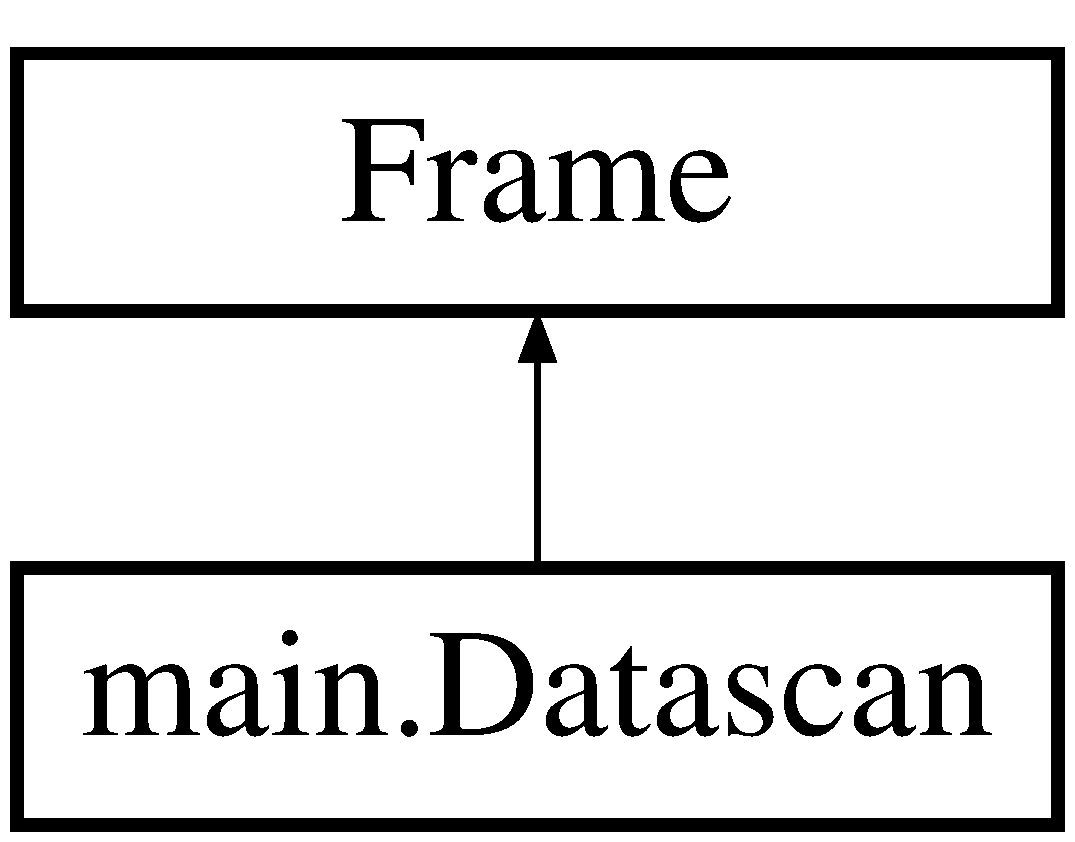
\includegraphics[height=2.000000cm]{classmain_1_1_datascan}
\end{center}
\end{figure}
\subsection*{Public Member Functions}
\begin{DoxyCompactItemize}
\item 
def \hyperlink{classmain_1_1_datascan_a75285f8f90631fe7661f29bb3e272fee}{\+\_\+\+\_\+init\+\_\+\+\_\+}
\item 
\hypertarget{classmain_1_1_datascan_a63b24a9e46917a900d419b7e4e9f1691}{}def {\bfseries browse} (self)\label{classmain_1_1_datascan_a63b24a9e46917a900d419b7e4e9f1691}

\item 
\hypertarget{classmain_1_1_datascan_a14ac37e12f6e1ec7ab378c3cbe2f15cb}{}def {\bfseries des} (self)\label{classmain_1_1_datascan_a14ac37e12f6e1ec7ab378c3cbe2f15cb}

\end{DoxyCompactItemize}
\subsection*{Public Attributes}
\begin{DoxyCompactItemize}
\item 
\hypertarget{classmain_1_1_datascan_a24941fbd92175dc228d9f396619e5a13}{}{\bfseries address}\label{classmain_1_1_datascan_a24941fbd92175dc228d9f396619e5a13}

\item 
\hypertarget{classmain_1_1_datascan_a79a379a932a86ad29673415ba630a764}{}{\bfseries l0}\label{classmain_1_1_datascan_a79a379a932a86ad29673415ba630a764}

\item 
\hypertarget{classmain_1_1_datascan_a448e8c3a009857e5a57de18429a1764d}{}{\bfseries b0}\label{classmain_1_1_datascan_a448e8c3a009857e5a57de18429a1764d}

\item 
\hypertarget{classmain_1_1_datascan_acc9117ed521eacea2240f642980f2950}{}{\bfseries title}\label{classmain_1_1_datascan_acc9117ed521eacea2240f642980f2950}

\end{DoxyCompactItemize}


\subsection{Constructor \& Destructor Documentation}
\hypertarget{classmain_1_1_datascan_a75285f8f90631fe7661f29bb3e272fee}{}\index{main\+::\+Datascan@{main\+::\+Datascan}!\+\_\+\+\_\+init\+\_\+\+\_\+@{\+\_\+\+\_\+init\+\_\+\+\_\+}}
\index{\+\_\+\+\_\+init\+\_\+\+\_\+@{\+\_\+\+\_\+init\+\_\+\+\_\+}!main\+::\+Datascan@{main\+::\+Datascan}}
\subsubsection[{\+\_\+\+\_\+init\+\_\+\+\_\+}]{\setlength{\rightskip}{0pt plus 5cm}def main.\+Datascan.\+\_\+\+\_\+init\+\_\+\+\_\+ (
\begin{DoxyParamCaption}
\item[{}]{self, }
\item[{}]{parent = {\ttfamily None}, }
\item[{}]{typestr = {\ttfamily None}, }
\item[{}]{title = {\ttfamily \textquotesingle{}\textquotesingle{}}}
\end{DoxyParamCaption}
)}\label{classmain_1_1_datascan_a75285f8f90631fe7661f29bb3e272fee}
\begin{DoxyVerb}:param parent: original file
:param typestr: string
:param title: course title
\end{DoxyVerb}
 

The documentation for this class was generated from the following file\+:\begin{DoxyCompactItemize}
\item 
main.\+py\end{DoxyCompactItemize}

\hypertarget{classmain_1_1_grad}{}\section{main.\+Grad Class Reference}
\label{classmain_1_1_grad}\index{main.\+Grad@{main.\+Grad}}
Inheritance diagram for main.\+Grad\+:\begin{figure}[H]
\begin{center}
\leavevmode
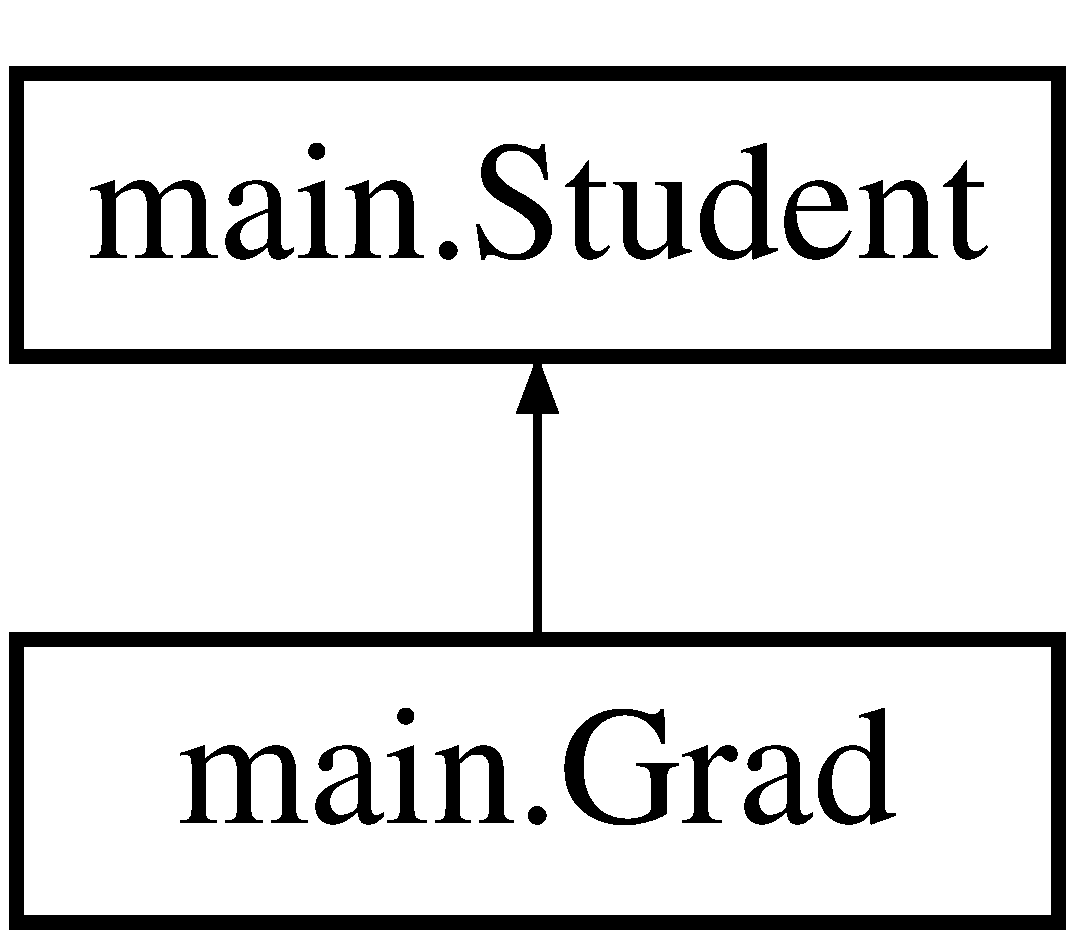
\includegraphics[height=2.000000cm]{classmain_1_1_grad}
\end{center}
\end{figure}
\subsection*{Public Member Functions}
\begin{DoxyCompactItemize}
\item 
def \hyperlink{classmain_1_1_grad_a3f6aa96bd1cf21f0b5997b766a823448}{\+\_\+\+\_\+init\+\_\+\+\_\+} (self, name, sid)
\item 
\hypertarget{classmain_1_1_grad_a325a69a0de8be8cb30fceab1c3f8c4d3}{}def {\bfseries \+\_\+\+\_\+repr\+\_\+\+\_\+} (self)\label{classmain_1_1_grad_a325a69a0de8be8cb30fceab1c3f8c4d3}

\end{DoxyCompactItemize}
\subsection*{Public Attributes}
\begin{DoxyCompactItemize}
\item 
\hypertarget{classmain_1_1_grad_a7b5d854c511c3adb0b5bc54d113af796}{}{\bfseries cou}\label{classmain_1_1_grad_a7b5d854c511c3adb0b5bc54d113af796}

\item 
\hypertarget{classmain_1_1_grad_a3f75233b7ee3d2f9071d6af45e8ae7e2}{}{\bfseries lan}\label{classmain_1_1_grad_a3f75233b7ee3d2f9071d6af45e8ae7e2}

\item 
\hypertarget{classmain_1_1_grad_acf2607e271077f049d9e98b432350e63}{}{\bfseries pl}\label{classmain_1_1_grad_acf2607e271077f049d9e98b432350e63}

\item 
\hypertarget{classmain_1_1_grad_aa88187797aeb6bd854c8342698378b1d}{}{\bfseries note}\label{classmain_1_1_grad_aa88187797aeb6bd854c8342698378b1d}

\end{DoxyCompactItemize}


\subsection{Constructor \& Destructor Documentation}
\hypertarget{classmain_1_1_grad_a3f6aa96bd1cf21f0b5997b766a823448}{}\index{main\+::\+Grad@{main\+::\+Grad}!\+\_\+\+\_\+init\+\_\+\+\_\+@{\+\_\+\+\_\+init\+\_\+\+\_\+}}
\index{\+\_\+\+\_\+init\+\_\+\+\_\+@{\+\_\+\+\_\+init\+\_\+\+\_\+}!main\+::\+Grad@{main\+::\+Grad}}
\subsubsection[{\+\_\+\+\_\+init\+\_\+\+\_\+(self, name, sid)}]{\setlength{\rightskip}{0pt plus 5cm}def main.\+Grad.\+\_\+\+\_\+init\+\_\+\+\_\+ (
\begin{DoxyParamCaption}
\item[{}]{self, }
\item[{}]{name, }
\item[{}]{sid}
\end{DoxyParamCaption}
)}\label{classmain_1_1_grad_a3f6aa96bd1cf21f0b5997b766a823448}
\begin{DoxyVerb}:param name: student name
:param sid: student id number
\end{DoxyVerb}
 

The documentation for this class was generated from the following file\+:\begin{DoxyCompactItemize}
\item 
main.\+py\end{DoxyCompactItemize}

\hypertarget{classmain_1_1_scrolled_text}{}\section{main.\+Scrolled\+Text Class Reference}
\label{classmain_1_1_scrolled_text}\index{main.\+Scrolled\+Text@{main.\+Scrolled\+Text}}
Inheritance diagram for main.\+Scrolled\+Text\+:\begin{figure}[H]
\begin{center}
\leavevmode
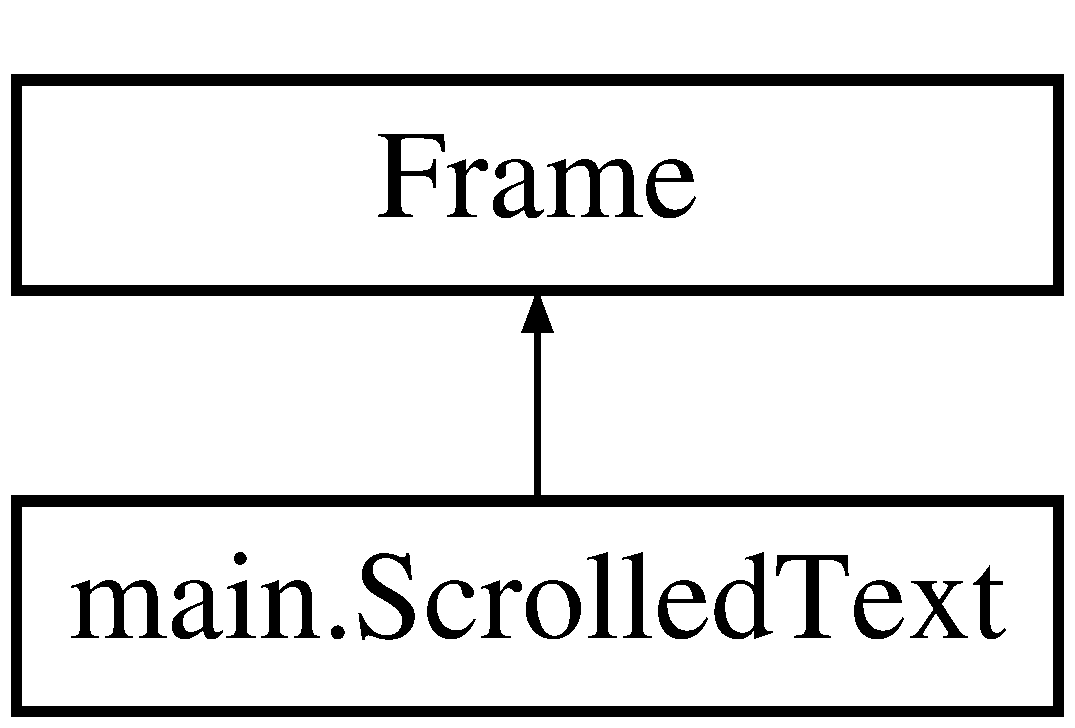
\includegraphics[height=2.000000cm]{classmain_1_1_scrolled_text}
\end{center}
\end{figure}
\subsection*{Public Member Functions}
\begin{DoxyCompactItemize}
\item 
\hypertarget{classmain_1_1_scrolled_text_a8dfda3dc2fe3ea57617aeb2dd3d7b6d5}{}def {\bfseries \+\_\+\+\_\+init\+\_\+\+\_\+}\label{classmain_1_1_scrolled_text_a8dfda3dc2fe3ea57617aeb2dd3d7b6d5}

\item 
\hypertarget{classmain_1_1_scrolled_text_a02b3adc55ed2f9c02b02afb7b9af7a2e}{}def {\bfseries makewidget} (self)\label{classmain_1_1_scrolled_text_a02b3adc55ed2f9c02b02afb7b9af7a2e}

\item 
\hypertarget{classmain_1_1_scrolled_text_a1f22f42049dc1afbca6b94b7f341788a}{}def {\bfseries settext} (self, text)\label{classmain_1_1_scrolled_text_a1f22f42049dc1afbca6b94b7f341788a}

\end{DoxyCompactItemize}
\subsection*{Public Attributes}
\begin{DoxyCompactItemize}
\item 
\hypertarget{classmain_1_1_scrolled_text_a64205b5ecc73fc73038b86d7058cade7}{}{\bfseries text}\label{classmain_1_1_scrolled_text_a64205b5ecc73fc73038b86d7058cade7}

\end{DoxyCompactItemize}


The documentation for this class was generated from the following file\+:\begin{DoxyCompactItemize}
\item 
main.\+py\end{DoxyCompactItemize}

\hypertarget{classmain_1_1_student}{}\section{main.\+Student Class Reference}
\label{classmain_1_1_student}\index{main.\+Student@{main.\+Student}}
Inheritance diagram for main.\+Student\+:\begin{figure}[H]
\begin{center}
\leavevmode
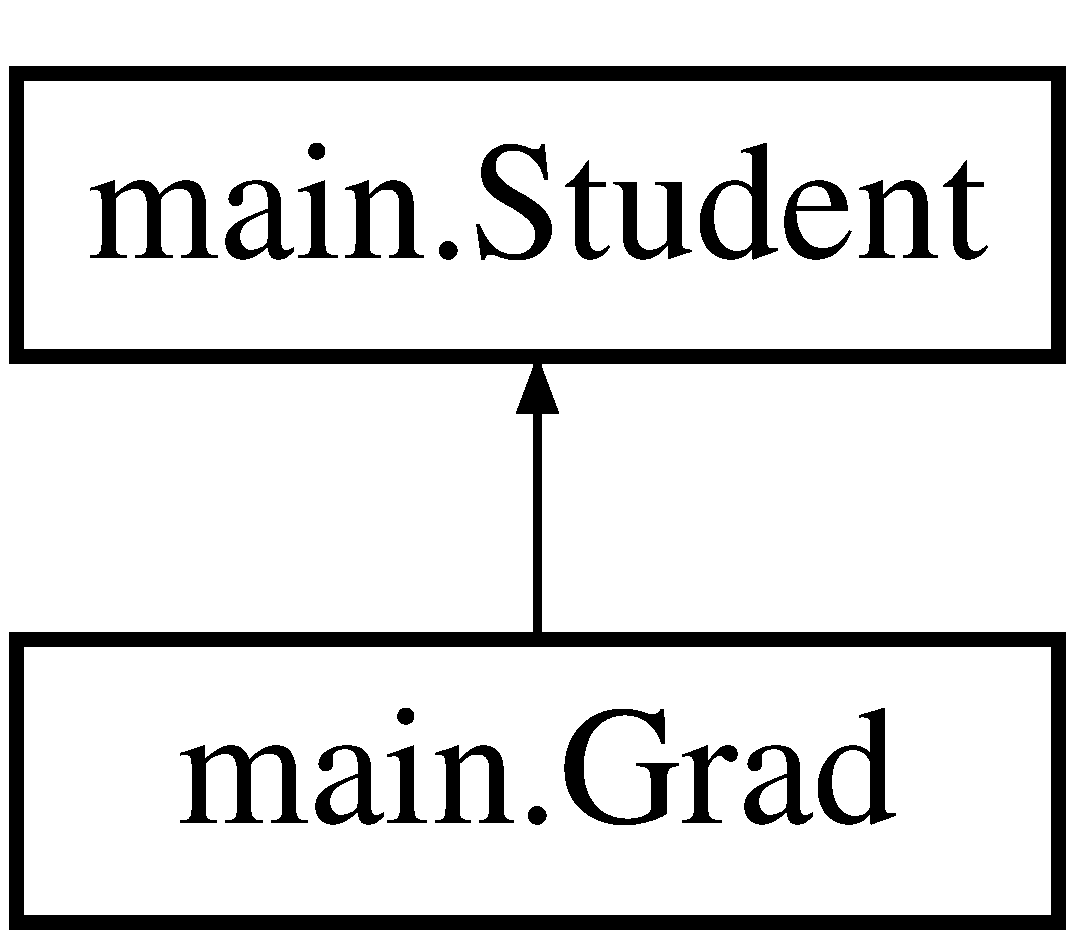
\includegraphics[height=2.000000cm]{classmain_1_1_student}
\end{center}
\end{figure}
\subsection*{Public Member Functions}
\begin{DoxyCompactItemize}
\item 
def \hyperlink{classmain_1_1_student_a495c5a676f26204f8e000e1194ed8110}{\+\_\+\+\_\+init\+\_\+\+\_\+}
\item 
\hypertarget{classmain_1_1_student_a5e0c2b9090e8b6f80e6c9d161ee84d97}{}def {\bfseries \+\_\+\+\_\+repr\+\_\+\+\_\+} (self)\label{classmain_1_1_student_a5e0c2b9090e8b6f80e6c9d161ee84d97}

\item 
def \hyperlink{classmain_1_1_student_a67de6c9f3d381d7234cef28bc0fadb21}{update} (self, day, bt)
\end{DoxyCompactItemize}
\subsection*{Public Attributes}
\begin{DoxyCompactItemize}
\item 
\hypertarget{classmain_1_1_student_a16e24ea558f049f03fca766b1fc64c65}{}{\bfseries name}\label{classmain_1_1_student_a16e24ea558f049f03fca766b1fc64c65}

\item 
\hypertarget{classmain_1_1_student_a2c8051e7ec636a7066252f839ab8fcb0}{}{\bfseries sid}\label{classmain_1_1_student_a2c8051e7ec636a7066252f839ab8fcb0}

\item 
\hypertarget{classmain_1_1_student_aded0368fbae736d7b6e1b5e1ccd1f339}{}{\bfseries stime}\label{classmain_1_1_student_aded0368fbae736d7b6e1b5e1ccd1f339}

\item 
\hypertarget{classmain_1_1_student_a9edbee6fe38c1511a44f61f0290bbebd}{}{\bfseries course}\label{classmain_1_1_student_a9edbee6fe38c1511a44f61f0290bbebd}

\item 
\hypertarget{classmain_1_1_student_a4a2bc23d3b945a9a8714d0d7aa4ca0e3}{}{\bfseries level}\label{classmain_1_1_student_a4a2bc23d3b945a9a8714d0d7aa4ca0e3}

\item 
\hypertarget{classmain_1_1_student_aa1e5c707385a7848fe00b5898f0a5409}{}{\bfseries ta}\label{classmain_1_1_student_aa1e5c707385a7848fe00b5898f0a5409}

\end{DoxyCompactItemize}


\subsection{Constructor \& Destructor Documentation}
\hypertarget{classmain_1_1_student_a495c5a676f26204f8e000e1194ed8110}{}\index{main\+::\+Student@{main\+::\+Student}!\+\_\+\+\_\+init\+\_\+\+\_\+@{\+\_\+\+\_\+init\+\_\+\+\_\+}}
\index{\+\_\+\+\_\+init\+\_\+\+\_\+@{\+\_\+\+\_\+init\+\_\+\+\_\+}!main\+::\+Student@{main\+::\+Student}}
\subsubsection[{\+\_\+\+\_\+init\+\_\+\+\_\+}]{\setlength{\rightskip}{0pt plus 5cm}def main.\+Student.\+\_\+\+\_\+init\+\_\+\+\_\+ (
\begin{DoxyParamCaption}
\item[{}]{self, }
\item[{}]{name, }
\item[{}]{sid, }
\item[{}]{level = {\ttfamily \textquotesingle{}UnderGrad\textquotesingle{}}}
\end{DoxyParamCaption}
)}\label{classmain_1_1_student_a495c5a676f26204f8e000e1194ed8110}
\begin{DoxyVerb}:param name: student's name
:param sid: student id number
:param level: undergradute or graduate
\end{DoxyVerb}
 

\subsection{Member Function Documentation}
\hypertarget{classmain_1_1_student_a67de6c9f3d381d7234cef28bc0fadb21}{}\index{main\+::\+Student@{main\+::\+Student}!update@{update}}
\index{update@{update}!main\+::\+Student@{main\+::\+Student}}
\subsubsection[{update(self, day, bt)}]{\setlength{\rightskip}{0pt plus 5cm}def main.\+Student.\+update (
\begin{DoxyParamCaption}
\item[{}]{self, }
\item[{}]{day, }
\item[{}]{bt}
\end{DoxyParamCaption}
)}\label{classmain_1_1_student_a67de6c9f3d381d7234cef28bc0fadb21}
\begin{DoxyVerb}The function update() add the busy time in each weekday.
The argument 'day' should be an integer in range(5) and 
argument 'bt' should be a tuple of the form (starttime, endtime)
:param day: returns day of the week
:param bt: returns time (hour:minute - hour:minute)
\end{DoxyVerb}
 

The documentation for this class was generated from the following file\+:\begin{DoxyCompactItemize}
\item 
main.\+py\end{DoxyCompactItemize}

\hypertarget{classmain_1_1_testcases}{}\section{main.\+Testcases Class Reference}
\label{classmain_1_1_testcases}\index{main.\+Testcases@{main.\+Testcases}}
Inheritance diagram for main.\+Testcases\+:\begin{figure}[H]
\begin{center}
\leavevmode
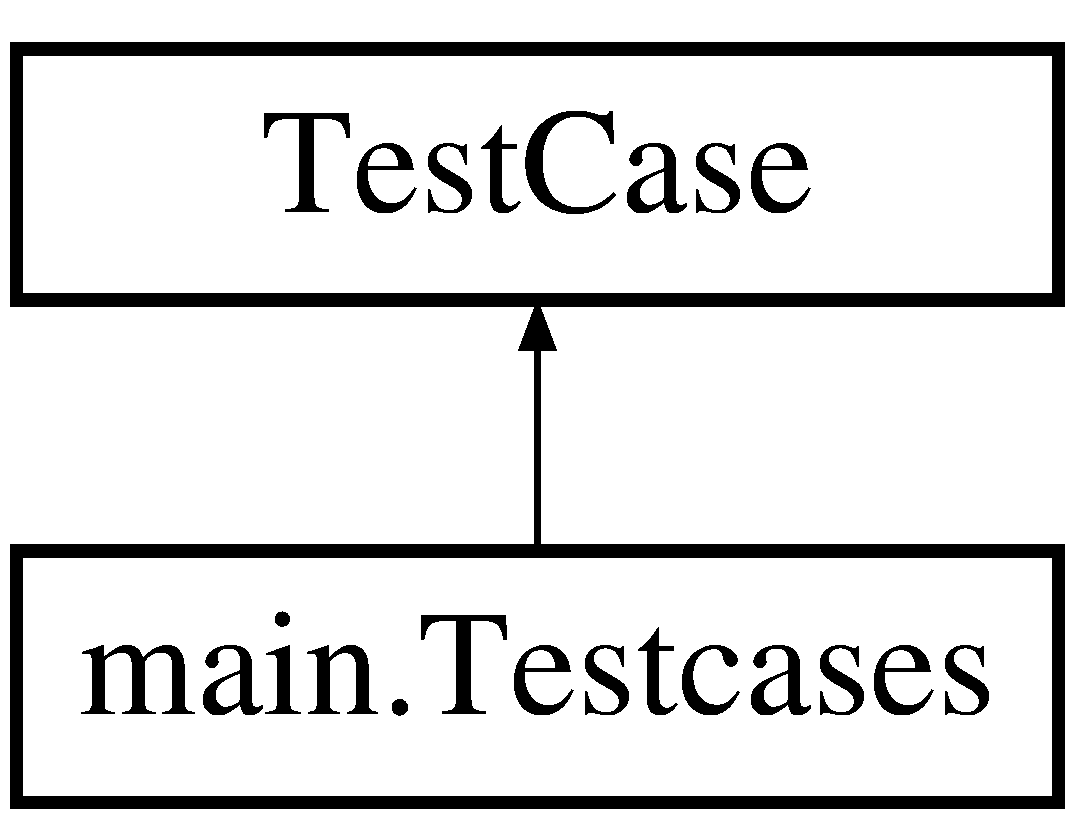
\includegraphics[height=2.000000cm]{classmain_1_1_testcases}
\end{center}
\end{figure}
\subsection*{Public Member Functions}
\begin{DoxyCompactItemize}
\item 
\hypertarget{classmain_1_1_testcases_a997fa2d1a3b7f5db020cfea3feedd300}{}def {\bfseries test\+\_\+strtime1} (self)\label{classmain_1_1_testcases_a997fa2d1a3b7f5db020cfea3feedd300}

\item 
\hypertarget{classmain_1_1_testcases_a5b29052d44fd7fb6d56fd13aeb792c56}{}def {\bfseries test\+\_\+strtime2} (self)\label{classmain_1_1_testcases_a5b29052d44fd7fb6d56fd13aeb792c56}

\item 
\hypertarget{classmain_1_1_testcases_afbad295f51840c173f3e7690935f9424}{}def {\bfseries test\+\_\+strime3} (self)\label{classmain_1_1_testcases_afbad295f51840c173f3e7690935f9424}

\item 
\hypertarget{classmain_1_1_testcases_acc017228af55dfa3c1c5e4f19de854c2}{}def {\bfseries test\+\_\+indig1} (self)\label{classmain_1_1_testcases_acc017228af55dfa3c1c5e4f19de854c2}

\item 
\hypertarget{classmain_1_1_testcases_ac7f2dbda87e66d24356900b3985ecb83}{}def {\bfseries test\+\_\+indig2} (self)\label{classmain_1_1_testcases_ac7f2dbda87e66d24356900b3985ecb83}

\item 
\hypertarget{classmain_1_1_testcases_ac576db962dbc29dcb11012f0b6c1629c}{}def {\bfseries test\+\_\+indig3} (self)\label{classmain_1_1_testcases_ac576db962dbc29dcb11012f0b6c1629c}

\item 
\hypertarget{classmain_1_1_testcases_aa8edc9b067e7c380bb6c6512f74c8b91}{}def {\bfseries test\+\_\+inalp1} (self)\label{classmain_1_1_testcases_aa8edc9b067e7c380bb6c6512f74c8b91}

\item 
\hypertarget{classmain_1_1_testcases_a45fa7057bf102da0a7780844291701d8}{}def {\bfseries test\+\_\+inalp2} (self)\label{classmain_1_1_testcases_a45fa7057bf102da0a7780844291701d8}

\item 
\hypertarget{classmain_1_1_testcases_a8b1c6ed146c459bffe7547507098ccfc}{}def {\bfseries test\+\_\+inalp3} (self)\label{classmain_1_1_testcases_a8b1c6ed146c459bffe7547507098ccfc}

\end{DoxyCompactItemize}


The documentation for this class was generated from the following file\+:\begin{DoxyCompactItemize}
\item 
main.\+py\end{DoxyCompactItemize}

\hypertarget{classmain_1_1_time}{}\section{main.\+Time Class Reference}
\label{classmain_1_1_time}\index{main.\+Time@{main.\+Time}}
\subsection*{Public Member Functions}
\begin{DoxyCompactItemize}
\item 
def \hyperlink{classmain_1_1_time_a0b98682596e4d5ae47dd39524b93dce1}{\+\_\+\+\_\+init\+\_\+\+\_\+}
\item 
def \hyperlink{classmain_1_1_time_aa50ec9969cd5e50958aacf9f664a8d43}{\+\_\+\+\_\+le\+\_\+\+\_\+} (self, x)
\item 
def \hyperlink{classmain_1_1_time_ab78ace96759768be0ab4b6784dd5e8c0}{\+\_\+\+\_\+ge\+\_\+\+\_\+} (self, x)
\item 
\hypertarget{classmain_1_1_time_a45e587371b8913b771d35a65742921cb}{}def {\bfseries \+\_\+\+\_\+repr\+\_\+\+\_\+} (self)\label{classmain_1_1_time_a45e587371b8913b771d35a65742921cb}

\item 
def \hyperlink{classmain_1_1_time_aad960c962856aceb0ce844fd5a25efe3}{dis} (self, y)
\end{DoxyCompactItemize}
\subsection*{Public Attributes}
\begin{DoxyCompactItemize}
\item 
\hypertarget{classmain_1_1_time_a4c963aaa96ef30517354ae7cab268f0c}{}{\bfseries time}\label{classmain_1_1_time_a4c963aaa96ef30517354ae7cab268f0c}

\end{DoxyCompactItemize}


\subsection{Constructor \& Destructor Documentation}
\hypertarget{classmain_1_1_time_a0b98682596e4d5ae47dd39524b93dce1}{}\index{main\+::\+Time@{main\+::\+Time}!\+\_\+\+\_\+init\+\_\+\+\_\+@{\+\_\+\+\_\+init\+\_\+\+\_\+}}
\index{\+\_\+\+\_\+init\+\_\+\+\_\+@{\+\_\+\+\_\+init\+\_\+\+\_\+}!main\+::\+Time@{main\+::\+Time}}
\subsubsection[{\+\_\+\+\_\+init\+\_\+\+\_\+}]{\setlength{\rightskip}{0pt plus 5cm}def main.\+Time.\+\_\+\+\_\+init\+\_\+\+\_\+ (
\begin{DoxyParamCaption}
\item[{}]{self, }
\item[{}]{hour = {\ttfamily 0}, }
\item[{}]{minute = {\ttfamily 0}}
\end{DoxyParamCaption}
)}\label{classmain_1_1_time_a0b98682596e4d5ae47dd39524b93dce1}
\begin{DoxyVerb}:param hour: inside the schedule text file; the hour of the class starting/ending
:param minute: inside the schedule text file; the minute of the class starting/ending
\end{DoxyVerb}
 

\subsection{Member Function Documentation}
\hypertarget{classmain_1_1_time_ab78ace96759768be0ab4b6784dd5e8c0}{}\index{main\+::\+Time@{main\+::\+Time}!\+\_\+\+\_\+ge\+\_\+\+\_\+@{\+\_\+\+\_\+ge\+\_\+\+\_\+}}
\index{\+\_\+\+\_\+ge\+\_\+\+\_\+@{\+\_\+\+\_\+ge\+\_\+\+\_\+}!main\+::\+Time@{main\+::\+Time}}
\subsubsection[{\+\_\+\+\_\+ge\+\_\+\+\_\+(self, x)}]{\setlength{\rightskip}{0pt plus 5cm}def main.\+Time.\+\_\+\+\_\+ge\+\_\+\+\_\+ (
\begin{DoxyParamCaption}
\item[{}]{self, }
\item[{}]{x}
\end{DoxyParamCaption}
)}\label{classmain_1_1_time_ab78ace96759768be0ab4b6784dd5e8c0}
\begin{DoxyVerb}:param x: used as a time comparison variable
\end{DoxyVerb}
 \hypertarget{classmain_1_1_time_aa50ec9969cd5e50958aacf9f664a8d43}{}\index{main\+::\+Time@{main\+::\+Time}!\+\_\+\+\_\+le\+\_\+\+\_\+@{\+\_\+\+\_\+le\+\_\+\+\_\+}}
\index{\+\_\+\+\_\+le\+\_\+\+\_\+@{\+\_\+\+\_\+le\+\_\+\+\_\+}!main\+::\+Time@{main\+::\+Time}}
\subsubsection[{\+\_\+\+\_\+le\+\_\+\+\_\+(self, x)}]{\setlength{\rightskip}{0pt plus 5cm}def main.\+Time.\+\_\+\+\_\+le\+\_\+\+\_\+ (
\begin{DoxyParamCaption}
\item[{}]{self, }
\item[{}]{x}
\end{DoxyParamCaption}
)}\label{classmain_1_1_time_aa50ec9969cd5e50958aacf9f664a8d43}
\begin{DoxyVerb}:param x: used as a time comparison variable
\end{DoxyVerb}
 \hypertarget{classmain_1_1_time_aad960c962856aceb0ce844fd5a25efe3}{}\index{main\+::\+Time@{main\+::\+Time}!dis@{dis}}
\index{dis@{dis}!main\+::\+Time@{main\+::\+Time}}
\subsubsection[{dis(self, y)}]{\setlength{\rightskip}{0pt plus 5cm}def main.\+Time.\+dis (
\begin{DoxyParamCaption}
\item[{}]{self, }
\item[{}]{y}
\end{DoxyParamCaption}
)}\label{classmain_1_1_time_aad960c962856aceb0ce844fd5a25efe3}
\begin{DoxyVerb}This function measures the distance between self and another time y.
:param y: used as a time comparison variable
\end{DoxyVerb}
 

The documentation for this class was generated from the following file\+:\begin{DoxyCompactItemize}
\item 
main.\+py\end{DoxyCompactItemize}

%--- End generated contents ---

% Index
\backmatter
\newpage
\phantomsection
\clearemptydoublepage
\addcontentsline{toc}{chapter}{Index}
\printindex

\end{document}
